\documentclass[10.5pt,scale=1.0,t,aspectratio=169,hyperref={pdfpagelabels=false}]{beamer}
%\usepackage[paperwidth=13.33in, paperheight=7.5in,top=.25in, bottom=.25in, left=.25in, right=.25in]{geometry}
%\geometry{papersize={13.33in,7.5in}}

%\usetheme{Dresden}
%\usetheme{Warsaw}

%Other themes
%https://hartwork.org/beamer-theme-matrix/

\usepackage{lipsum}
\usepackage{color}

\usepackage{amsfonts}
\usepackage{amsmath,mathtools}
\usepackage{mathrsfs}
\usepackage{array}
\usepackage{algorithm}
\usepackage{hyperref}
\usepackage[spanish,es-nodecimaldot]{babel}
\usepackage[utf8]{inputenc}
%\usepackage{intcalc}
\usepackage{graphicx}
\usepackage{multicol}
%\usepackage{authblk}
\usepackage{multirow}
\usepackage{enumitem}
\usepackage[document]{ragged2e}

\usepackage[absolute,overlay]{textpos}
\textblockorigin{0mm}{0mm} 

\usefonttheme[onlymath]{serif}
%\usepackage{epstopdf}
\usepackage{verbatim}
\usepackage{cite}
%\usepackage[texcoord,grid,gridunit=mm,gridcolor=red!10,subgridcolor=green!10]{eso-pic}




\newenvironment{conditions}[1][where:]
{#1 \begin{tabular}[t]{>{$}l<{$} @{${}={}$} l}}
	{\end{tabular}\\[\belowdisplayskip]}


\newcolumntype{L}{>{$}l<{$}} % math-mode version of "l" column type


\newcounter{saveenumi}
\newcommand{\seti}{\setcounter{saveenumi}{\value{enumi}}}
\newcommand{\conti}{\setcounter{enumi}{\value{saveenumi}}}

\setbeamertemplate{bibliography item}{\insertbiblabel}


\hypersetup{colorlinks=true,
	linkcolor=blue,
	linktoc=all,				
	citecolor=blue,
	urlcolor=red,
	pdftitle={FUNDAMENTOS DE AUTOMATIZACIÓN Y CONTROL},
	pdfauthor={Santiago Rúa Pérez},
	pdfcreator={Santiago Rúa Pérez}}


\definecolor{GreenDark}{rgb}{0.0, 0.60, 0.0}
\definecolor{RedDark}{rgb}{183, 0.0, 0.0}
\definecolor{BlueDark}{rgb}{0.0, 0.0, 167}
\definecolor{BlueLight}{rgb}{0.2, 0.451, 0.517}


\graphicspath{{imag/}}

\newcommand{\Ho}{$H_{0}$}
\newcommand{\Ha}{$H_{a}$}
\newcommand{\Nota}{{\bf Nota: }}
\newcolumntype{P}[1]{>{\centering\arraybackslash}p{#1}}
\newcolumntype{M}[1]{>{\centering\arraybackslash}m{#1}}

\newcommand{\less}{<}
\newcommand{\greater}{>}


\setlength{\parindent}{1em}
\setlength{\parskip}{.6em}
\renewcommand{\baselinestretch}{.9}

%%%%    C environment    ---------------- %%%%%%%%%%%%%%%.
\usepackage{listings}
\usepackage{xcolor}
\definecolor{mGreen}{rgb}{0,0.6,0}
\definecolor{mGray}{rgb}{0.5,0.5,0.5}
\definecolor{mPurple}{rgb}{0.58,0,0.82}
\definecolor{backgroundColour}{rgb}{0.95,0.95,0.92}

\lstdefinestyle{CStyle}{
	backgroundcolor=\color{backgroundColour},   
	commentstyle=\color{mGreen},
	keywordstyle=\color{magenta},
	numberstyle=\tiny\color{mGray},
	stringstyle=\color{mPurple},
	basicstyle=\tiny,
	breakatwhitespace=false,         
	breaklines=true,                 
	captionpos=b,                    
	keepspaces=true,                 
	numbers=left,                    
	numbersep=5pt,                  
	showspaces=false,                
	showstringspaces=false,
	showtabs=false,                  
	tabsize=2,
	language=C
}
%%--------------------------------------------------------------------------


\title{Electrónica Digital II}   
\author{Santiago Rúa Pérez, PhD.} 
\date{\today} 

\setlength{\TPHorizModule}{\textwidth}
\setlength{\TPVertModule}{\textwidth}

\newcommand{\btVFill}{\vskip0pt plus 1filll}


\setbeamertemplate{sidebar right}{}
\setbeamertemplate{footline}
{
	\leavevmode%
	\hbox{%
		\begin{beamercolorbox}[wd=.333333\paperwidth,ht=2.25ex,dp=1ex,center]{author in head/foot}%
			\usebeamerfont{author in head/foot}\insertshortauthor
		\end{beamercolorbox}%
		\begin{beamercolorbox}[wd=.333333\paperwidth,ht=2.25ex,dp=1ex,center]{title in head/foot}%
			\usebeamerfont{title in head/foot}\insertshorttitle
	\end{beamercolorbox}}%
	\vskip0pt%
}
\makeatother

%\frame{\frametitle{Tabla de contenidos}\tableofcontents} 
\begin{document}
%%%%%%%%%%%%%%%%%% FRAME %%%%%%%%%%%%%%%%%%%%%%%%%%
\begin{frame}
	\titlepage
\end{frame}
%%%%%%%%%%%%%%%%% FRAME START %%%%%%%%%%%%%%%%%%%%%%%%%%
\frame{
%\frametitle{}
\begin{center}
\LARGE \textcolor{blue}{CONCEPTOS BÁSICOS DE PROGRAMACIÓN EN C}
\end{center}
}
%%%%%%%%%%%%%%%%% FRAME START %%%%%%%%%%%%%%%%%%%%%%%%%%

%%%%%%%%%%%%%%%%% FRAME %%%%%%%%%%%%%%%%%%%%%%%%%%
\frame{
\frametitle{Introduccion a programación en C}
{\bf Objetivos}
\begin{itemize}
\item Entender los objetivos Básicos de los computadores.
\item Entender los diferentes tipos de lenguaje de programación.
\item Ambiente tipico de c.
\item Estructuras condicionadas. 

\end{itemize}
}
%%%%%%%%%%%%%%%%% FRAME %%%%%%%%%%%%%%%%%%%%%%%%%%

%%%%%%%%%%%%%%%%% FRAME %%%%%%%%%%%%%%%%%%%%%%%%%%
\frame{
	\begin{figure}
		\centering
		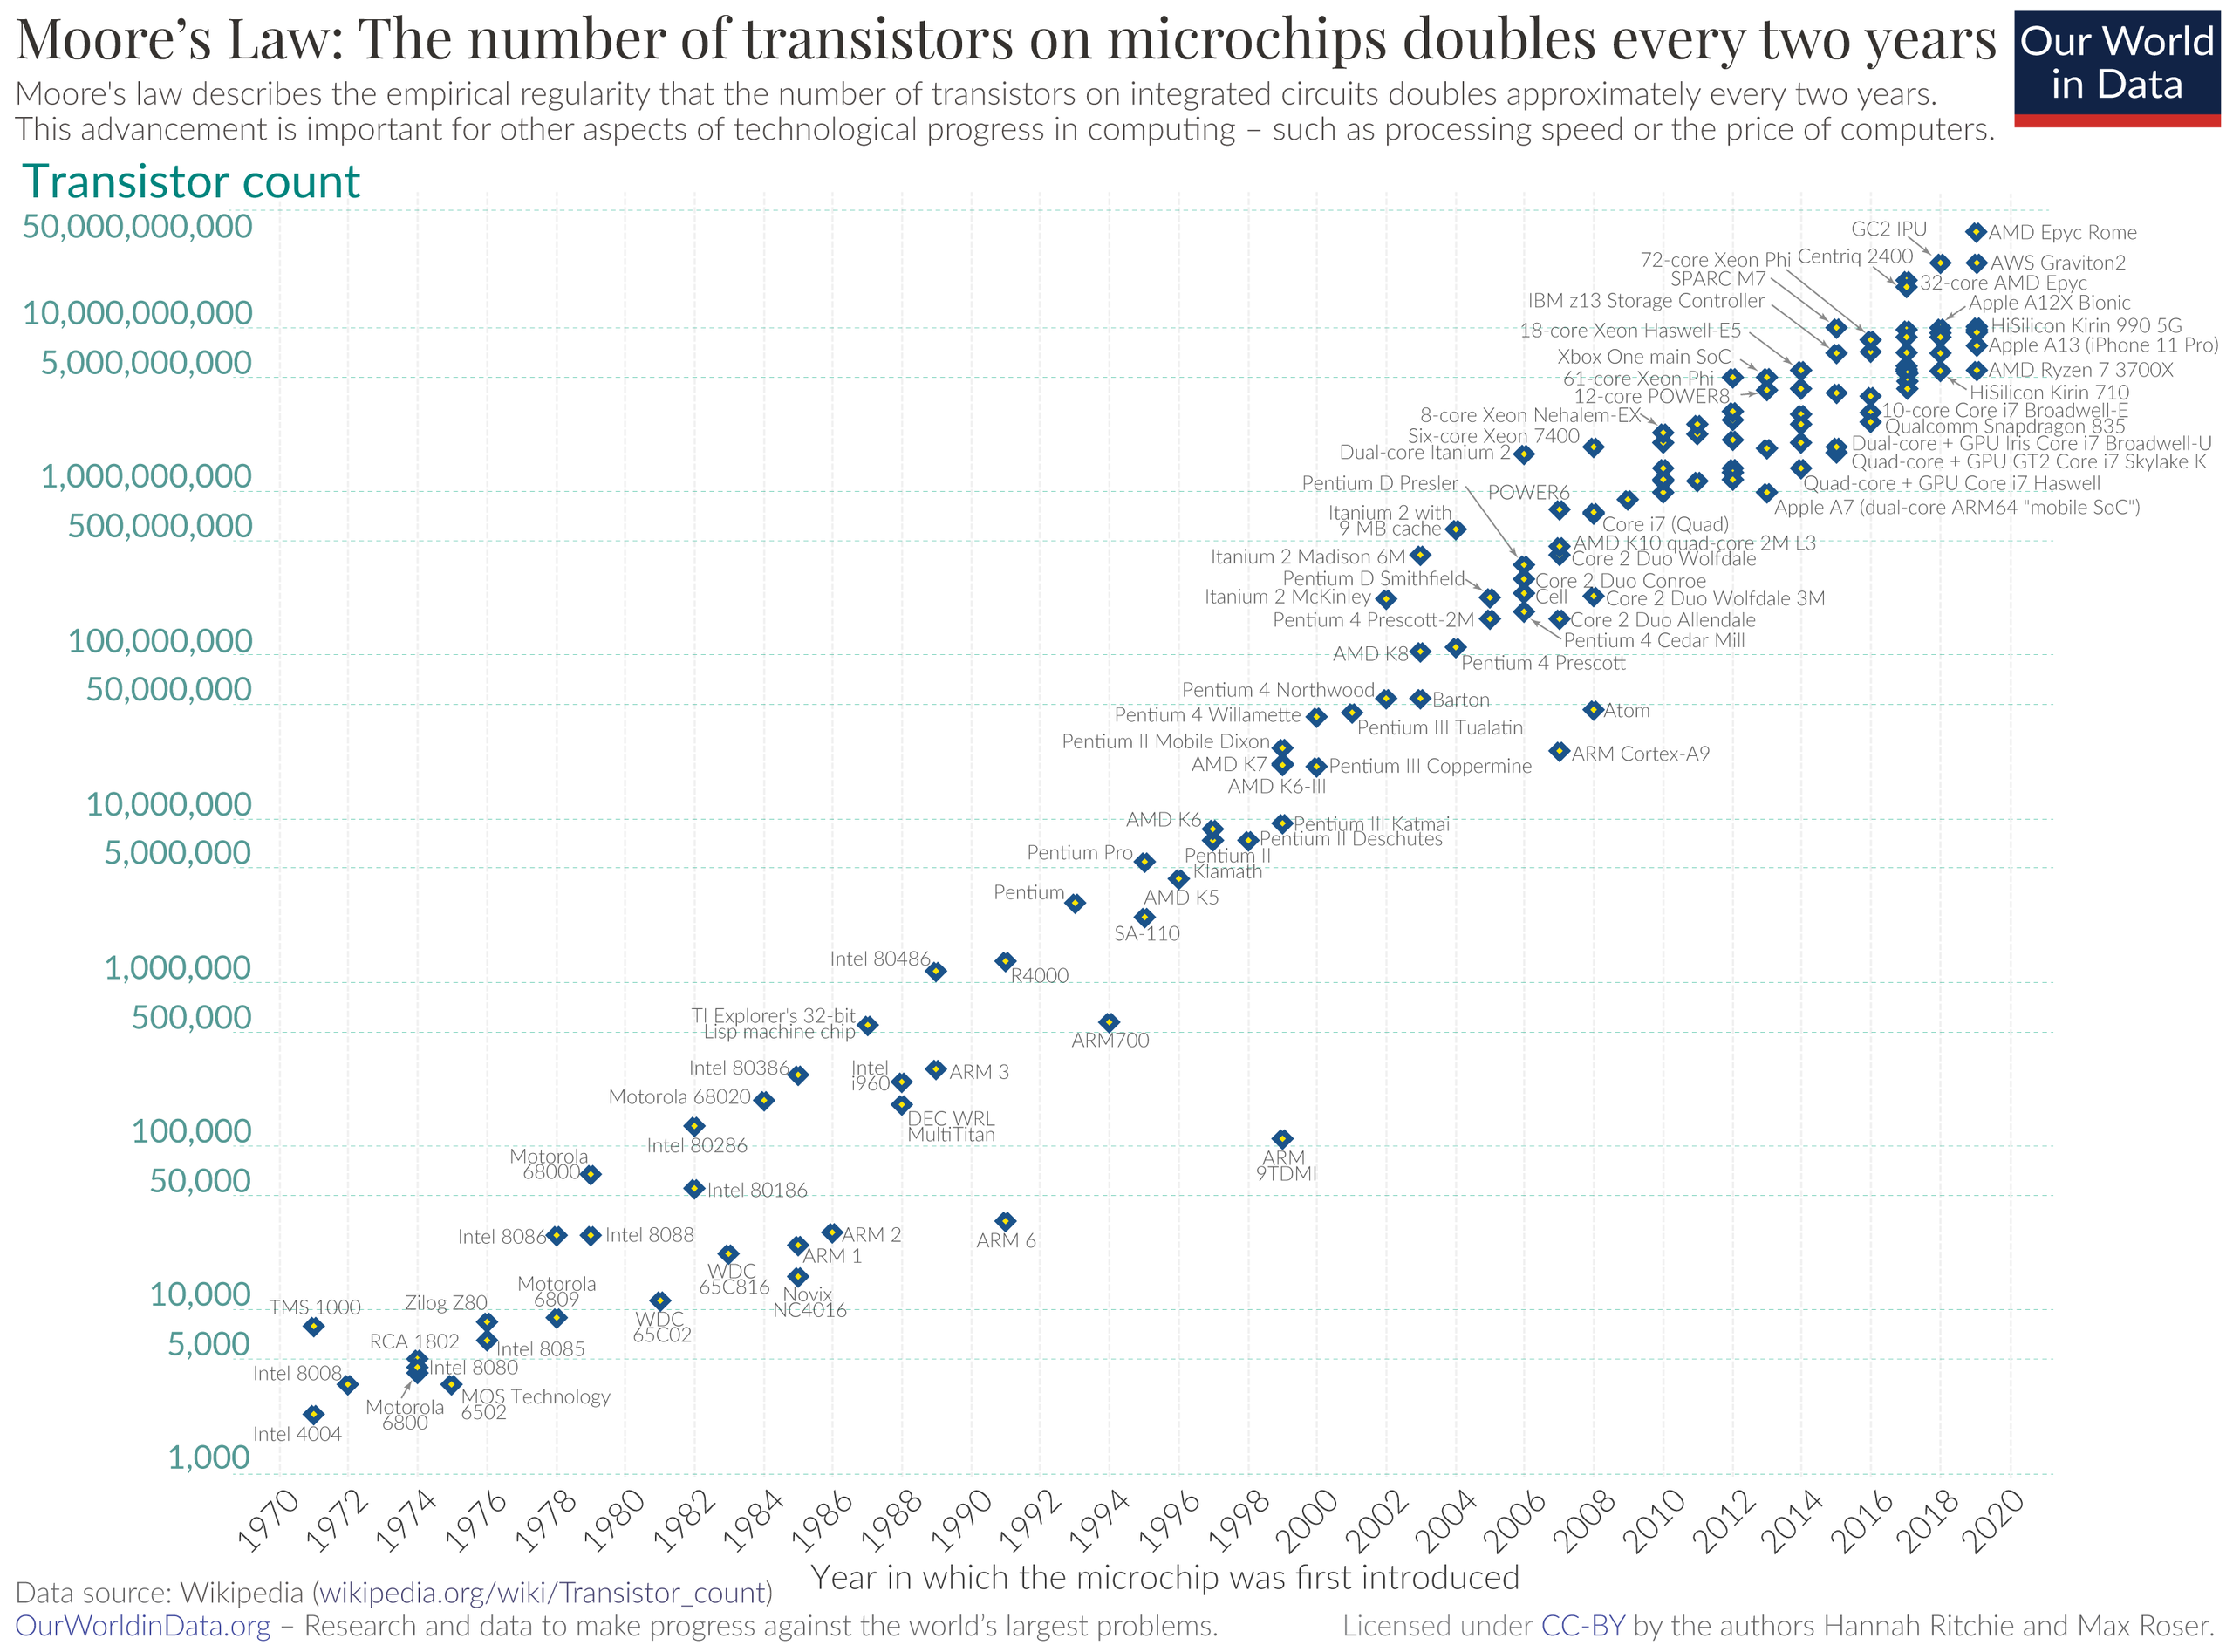
\includegraphics[width=10cm]{MooresLaw}
	\end{figure}

}
%%%%%%%%%%%%%%%%% FRAME %%%%%%%%%%%%%%%%%%%%%%%%%%
\begin{frame}
\frametitle{Arquitectura de computadores}
	\begin{figure}
		\centering
		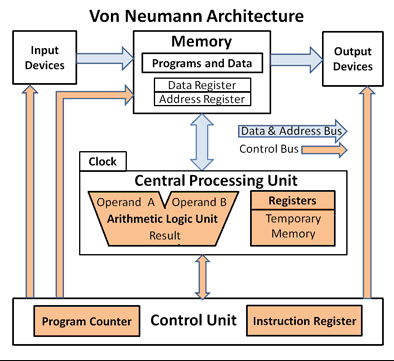
\includegraphics[width=7cm]{ComputerArchitecture}
	\end{figure}
\end{frame}

%%%%%%%%%%%%%%%%% FRAME %%%%%%%%%%%%%%%%%%%%%%%%%%
\begin{frame}
	\frametitle{Lenguajes de programación}
	\begin{columns}
		\column{0.3\linewidth}
		\begin{block}{\small Lenguaje de Máquina}
			\justifying
			\small
			\begin{itemize}
				\item Depende de la máquina.
				\item Cadena de números.
				\item \texttt{010011110}
			\end{itemize}
		\end{block}
		
		\column{0.3\linewidth}
		\begin{block}{\small Ensamblador}
			\justifying
			\small
			\begin{itemize}
				\item Abreviaciones en inglés.
				\item Base de lenguaje.
				\item Mas facil de entender por humanos.
				\item \texttt{load, add, store}
			\end{itemize}
		\end{block}
	
		\column{0.3\linewidth}
		\begin{block}{\small Alto nivel}
			\justifying
			\small
			\begin{itemize}
				\item Mas facil de programar.
				\item Exportabilidad. 
				\item \texttt{grossPay = basePay + overTimePay}
			\end{itemize}
		\end{block}
	\end{columns}
\end{frame}
%%%%%%%%%%%%%%%%% FRAME %%%%%%%%%%%%%%%%%%%%%%%%%%
\begin{frame}
	\frametitle{Pseudocódigo}
	Como seria el pseudocodigo para calcular el salario a pagar a un empleador?
\end{frame}

%%%%%%%%%%%%%%%%% FRAME %%%%%%%%%%%%%%%%%%%%%%%%%%
\begin{frame}
	\frametitle{Lenguaje de Programación C}
	\begin{figure}
		\centering
		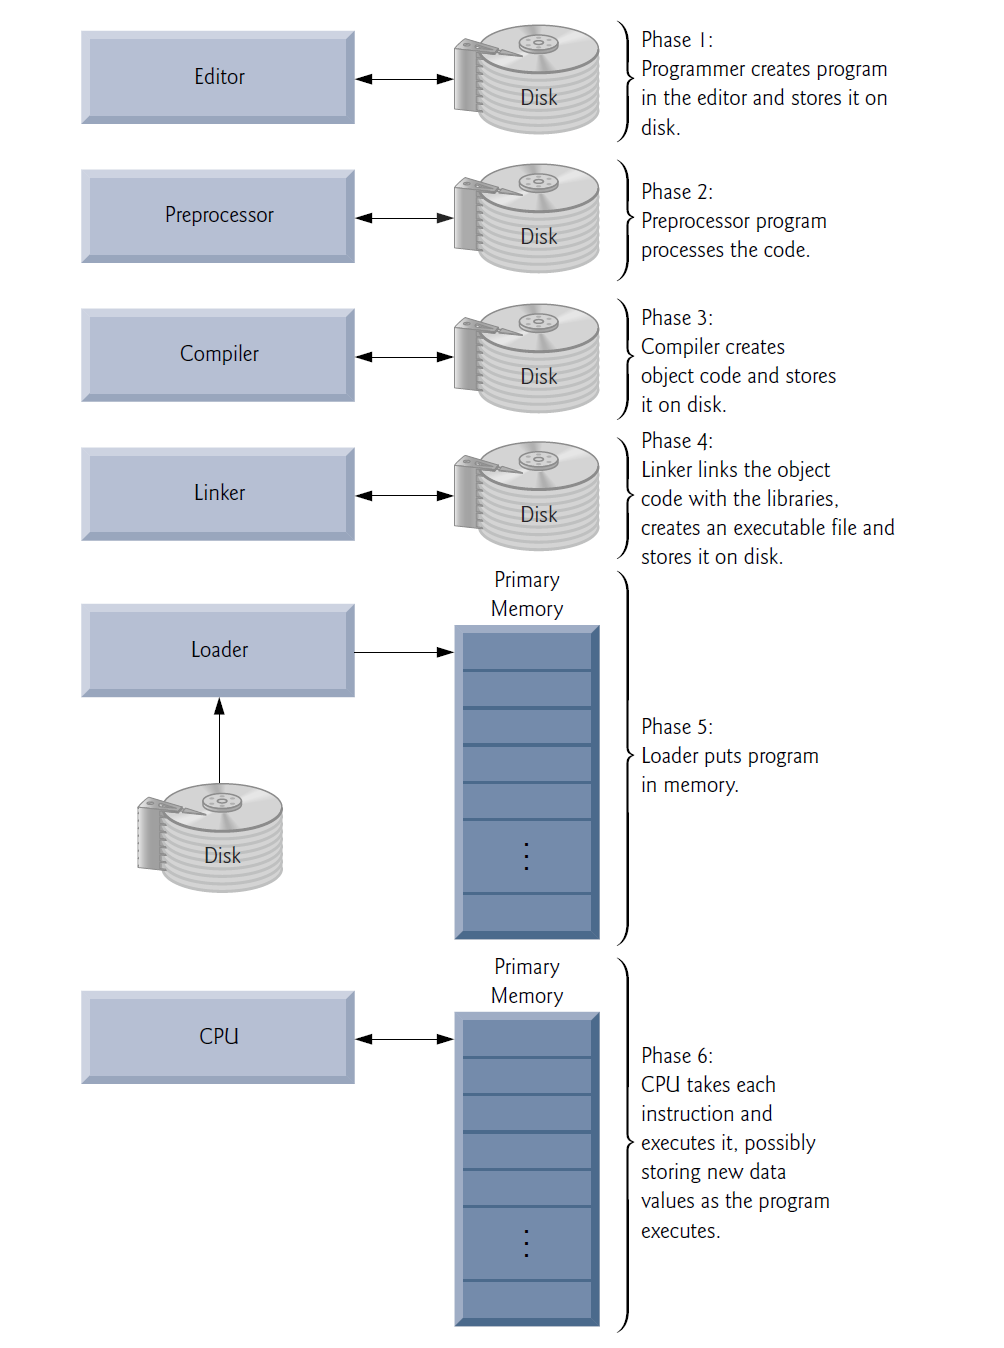
\includegraphics[width=6cm]{ProgramacionCEstructura}
	\end{figure}
\end{frame}
%%%%%%%%%%%%%%%%% FRAME %%%%%%%%%%%%%%%%%%%%%%%%%%
\begin{frame}[fragile]
	\frametitle{Primer Programa en C}
	
	Imprimir en consola la frase: `Hola Mundo'
	
	\begin{lstlisting}[style=CStyle]
		// Primer programa en C
		
		// Incluir libreria de salidas y entradas estandar
		#include <stdio.h>
		
		// Funcion donde comienza la ejecucion del programa
		int main(void)
		{
			printf("Hello World!"); 
		} // Fin de la funcion
	\end{lstlisting}
	
\end{frame}
%%%%%%%%%%%%%%%%% FRAME %%%%%%%%%%%%%%%%%%%%%%%%%%
\begin{frame}[fragile]
	\frametitle{Segundo Programa en C}
	
	Solicitar dos números enteros y devolver la suma de los mismos. 
	
	\begin{lstlisting}[style=CStyle]
		// Segundo programa en C
		
		// Incluir libreria de salidas y entradas estandar
		#include <stdio.h>
		
		// Funcion donde comienza la ejecucion del programa
		int main(void)
		{
			// Declaracion de variables
			int integer1;
			int integer2;
			
			// Almacenamiento de los numero dados por el usuario
			printf("Ingrese el primer entero\n");
			scanf("% d",&integer1);
			
			printf("Ingrese el segundo entero\n");
			scanf("% d",&integer2);
			
			int sum;
			sum = integer1 + integer2;
	
			printf("La suma es %d\n",sum); 
		} // Fin de la funcion
	\end{lstlisting}
\end{frame}

%%%%%%%%%%%%%%%%% FRAME %%%%%%%%%%%%%%%%%%%%%%%%%%
\frame{
	\frametitle{Aritmética en C}
		\begin{figure}
			\centering
			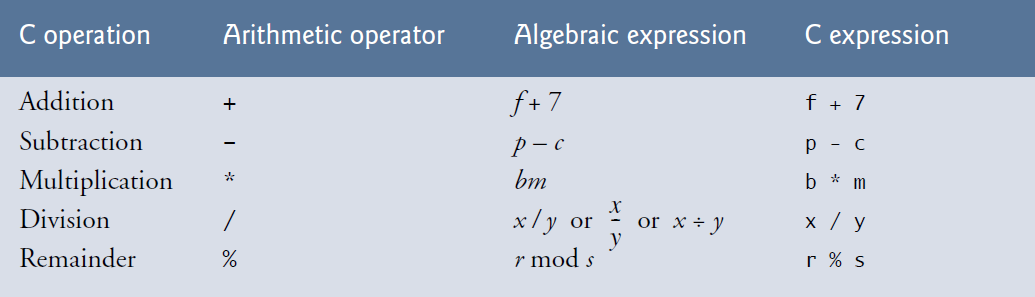
\includegraphics[width=8cm]{OperacionesEnC}
		\end{figure}
	
	\begin{figure}
		\centering
		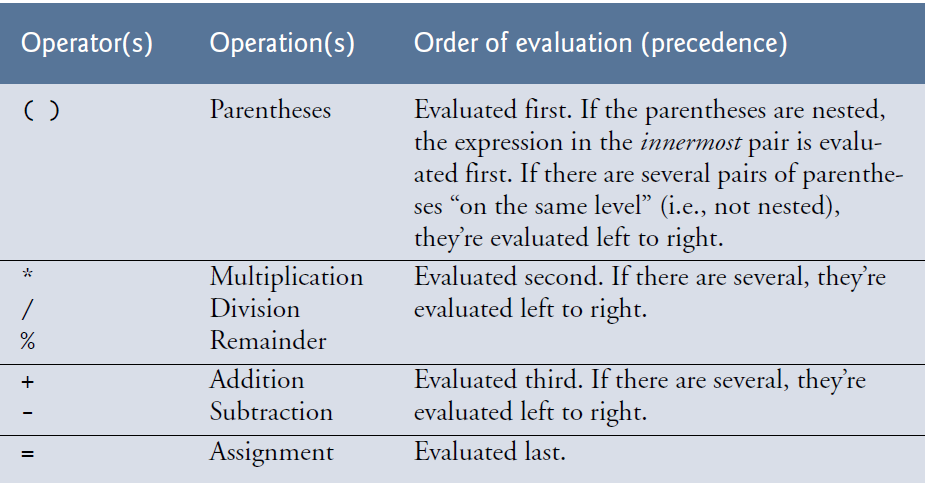
\includegraphics[width=8cm]{PrecedenciaOperadores}
	\end{figure}
	
}

%%%%%%%%%%%%%%%%% FRAME %%%%%%%%%%%%%%%%%%%%%%%%%%
\frame{
	\frametitle{Operadores de relación en C}
	\begin{figure}
		\centering
		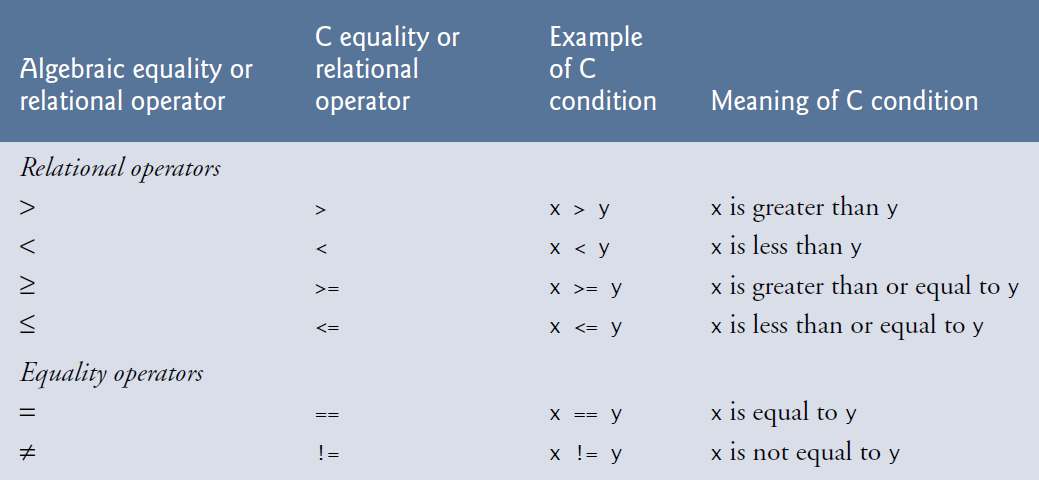
\includegraphics[width=8cm]{OperadoresRelacion}
	\end{figure}
	
}

%%%%%%%%%%%%%%%%% FRAME %%%%%%%%%%%%%%%%%%%%%%%%%%
\begin{frame}
	\frametitle{Palabras reservadas en C}
	\begin{figure}
		\centering
		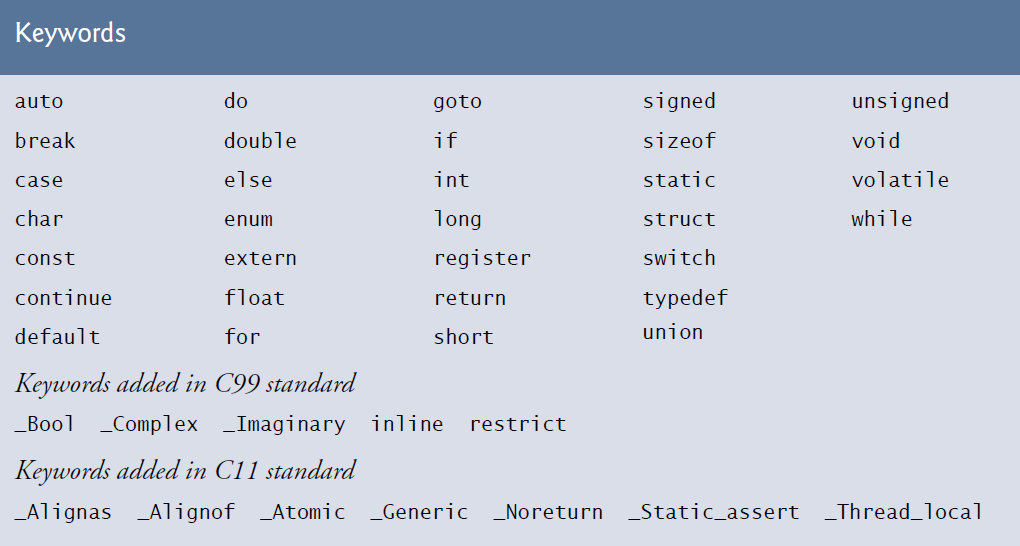
\includegraphics[width=8cm]{KeywordsC}
	\end{figure}
	
\end{frame}
%%%%%%%%%%%%%%%%% FRAME %%%%%%%%%%%%%%%%%%%%%%%%%%
\begin{frame}
	\frametitle{Ejemplos en C}
	\begin{itemize}
		\item Hacer un programa que le solicite al usuario tres enteros y obtenga la multiplicacion.
		\item Valide si dos números $a$ y $b$ son divisibles entre ellos.
		\item Encuentre los errores en la imagen.
	\end{itemize}
	\begin{figure}
		\centering
		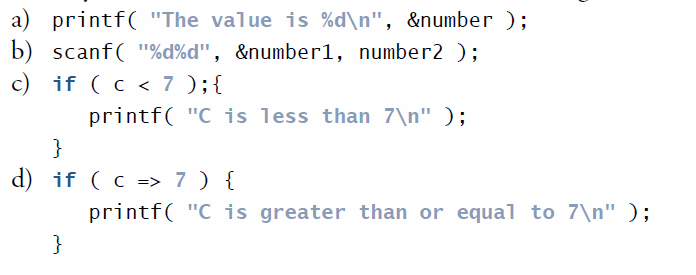
\includegraphics[width=8cm]{ErrorEjemplo}
	\end{figure}
\end{frame}

%%%%%%%%%%%%%%%%% FRAME %%%%%%%%%%%%%%%%%%%%%%%%%%
\begin{frame}
	\frametitle{Operadores de asignación}
	El operador de asignación de valor es $=$. Las operaciones tipicas son:
	\[
		variable = variable \ operador \ expresion
	\]
	\begin{figure}
		\centering
		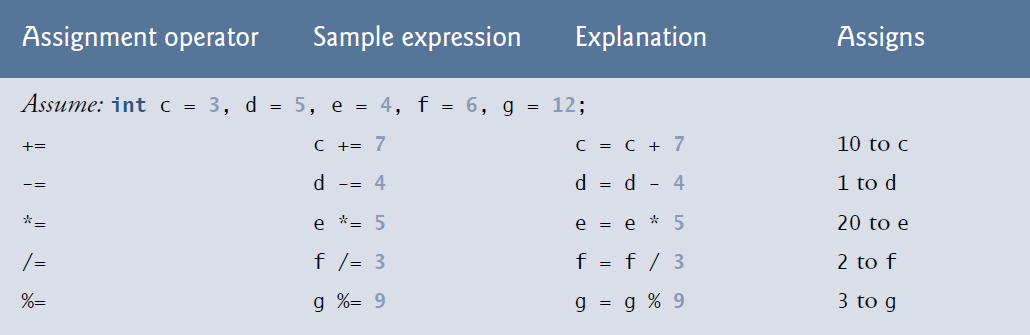
\includegraphics[width=7cm]{Operaciones}
	\end{figure}
	\begin{figure}
		\centering
		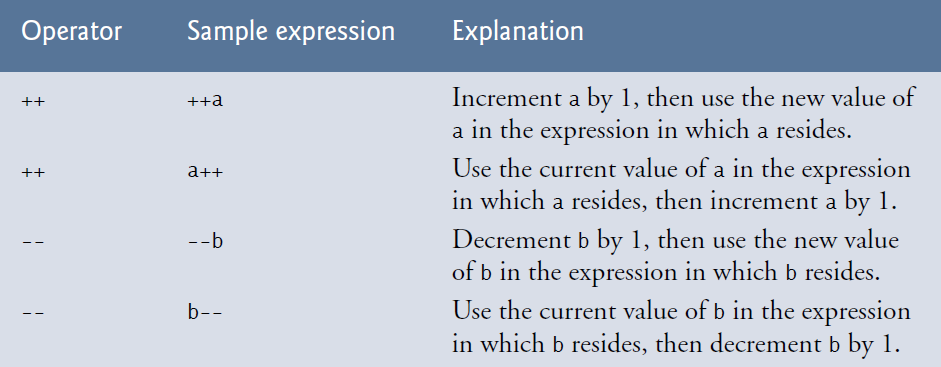
\includegraphics[width=7cm]{IncrementoDecremento}
	\end{figure}
\end{frame}


%%%%%%%%%%%%%%%%% FRAME %%%%%%%%%%%%%%%%%%%%%%%%%%
\begin{frame}
	\frametitle{Estructuras de control}
	\textcolor{blue}{\large Estructura If} \\
	Este tipo de instrucción es utilizado para seleccionar entre dos opciones
	
	\begin{columns}
		\column{0.3\linewidth}
		\begin{block}{\small If ...}
			\justifying
			Si la nota de un estudiantes es mayor a 3, entonces ganó el curso. 
		\end{block}
		
		\column{0.3\linewidth}
		\begin{block}{\small If ... else}
			\justifying
			Si la nota de un estudiantes es mayor a 3, entonces ganó el curso, sino perdio. 
		\end{block}
	
		\column{0.3\linewidth}
		\begin{block}{\small ?:}
			\justifying
			Operador condicional es ternario. 
			puts( grade >= 60 ? "Passed" : "Failed" ) 
		\end{block}
	\end{columns}
\end{frame}

%%%%%%%%%%%%%%%%% FRAME %%%%%%%%%%%%%%%%%%%%%%%%%%
\begin{frame}[fragile]
	\frametitle{Ejemplo operadores}
	
	Encuentre la relación entre dos números enteros. 
	
	\begin{lstlisting}[style=CStyle]
		// Using if statements, relational
		// operators, and equality operators.
		#include <stdio.h>
		
		// function main begins program execution
		int main( void )
		{
			printf( "Enter two integers, and I will tell you\n" );
			printf( "the relationships they satisfy: " );
			
			int num1; // first number to be read from user
			int num2; // second number to be read from user
			
			scanf( "% d % d", &num1, &num2 ); // read two integers	
			if ( num1 == num2 ) {
				printf( "%d is equal to % d\n", num1, num2 );
			}
			if ( num1 != num2 ) {
				printf( "% d is not equal to % d\n", num1, num2 );
			} // end if
			if ( num1 < num2 ) {
				printf( "% d is less than % d\n", num1, num2 );
			} //
			if ( num1 > num2 ) {
				printf( "% d is greater than % d\n", num1, num2 );
			} // end if
		}
	\end{lstlisting}
	
\end{frame}

%%%%%%%%%%%%%%%%% FRAME %%%%%%%%%%%%%%%%%%%%%%%%%%
\begin{frame}
	\frametitle{Estructuras condicionales}
	\textcolor{blue}{\large If anidados} \\
	\begin{figure}
		\centering
		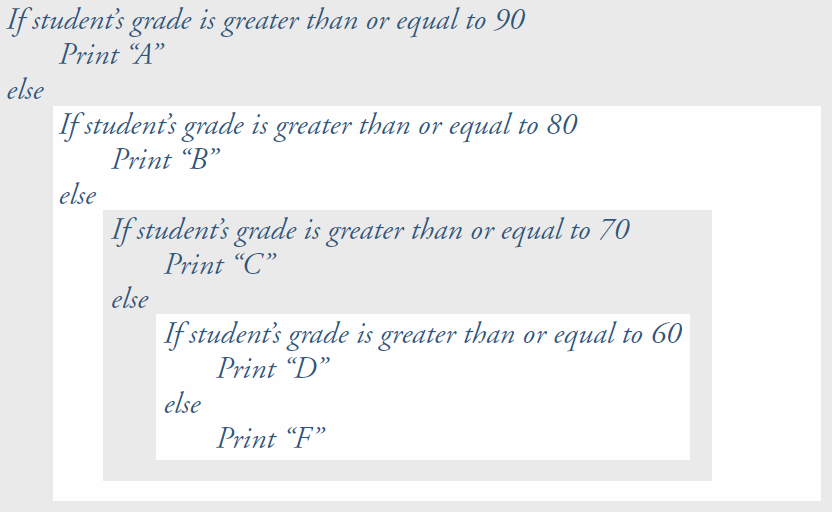
\includegraphics[width=8cm]{IfAnidado}
	\end{figure}	
\end{frame}

%%%%%%%%%%%%%%%%% FRAME %%%%%%%%%%%%%%%%%%%%%%%%%%
\begin{frame}[fragile]
	\frametitle{If anidados en C - ejemplo}
	
	Código en C.
	
	\begin{lstlisting}[style=CStyle]
		if ( grade >= 90 ) {
			puts( "A" );
		} // end if
		else if ( grade >= 80 ) {
			puts( "B" );
		} // end else if
		else if ( grade >= 70 ) {
			puts( "C" );
		} // end else if
		else if ( grade >= 60 ) {
			puts( "D" );
		} // end else if
		else {
			puts( "F" );
		} // end else
	\end{lstlisting}
	
\end{frame}


%%%%%%%%%%%%%%%%% FRAME %%%%%%%%%%%%%%%%%%%%%%%%%%
\begin{frame}
	\frametitle{Estructuras condicionales}
	\textcolor{blue}{\large Switch... case..} \\
	Es una estructura utilizada para la selección multiple. Su estructura es
	\begin{figure}
		\centering
		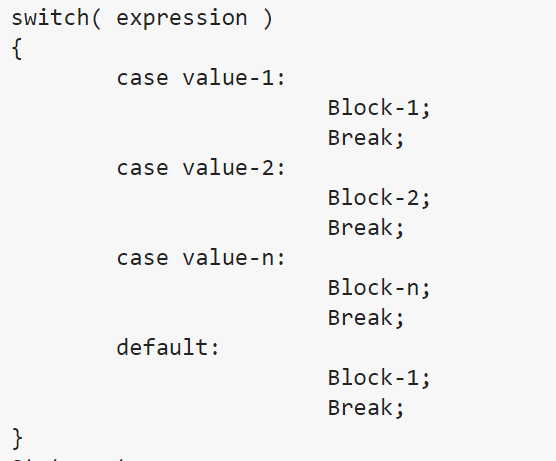
\includegraphics[width=5cm]{SwitchStructure}
	\end{figure}	
\end{frame}

%%%%%%%%%%%%%%%%% FRAME %%%%%%%%%%%%%%%%%%%%%%%%%%
\begin{frame}
	\frametitle{Estructuras condicionales}
	\textcolor{blue}{\large Ejemplos} \\
	\begin{itemize}
		\item Hacer un programa en C que solicite dos numeros flotantes. Unas vez ingresado los numeros flotantes, imprimir al usuario cuatro opciones de operaciones dadas asi: A. Suma, B. resta, C. Multiplicacion, D. Division. Una vez seleccionada la operación el programa retorna el valor de dicha operación.
		\item Una empresa tiene que llenar un formato de los impuestos a recolectar de acuerdo al mes de ventas. Hacer un programa que solicite el mes que va a generar los impuestos, las ventas de dicho mes, y calcules los impuestos del municipio (4\%) y los de la nación (5\%). 
		\item Haga un programa en C que cálcule cuanto se le consigna a una persona dado el salario acordado. Recuerde que a las persona se le debe deducir salud y pension, 4\% cada uno. 
	\end{itemize}	
\end{frame}


%%%%%%%%%%%%%%%%% FRAME %%%%%%%%%%%%%%%%%%%%%%%%%%
\frame{
\begin{center}
	\LARGE \textcolor{blue}{CONCEPTOS BÁSICOS DE PROGRAMACIÓN EN C}
\end{center}

\begin{center}
	\LARGE \textcolor{blue}{GRACIAS}
\end{center}
}

%%%%%%%%%%%%%%%%%%%%%%%%%%%%%%%%%%%%%%%%%%%%%%%%%%%%%%%%%%%%%%%%%%%%%%%%%%%%%%%%%%%%%%%%%%%%%%%%%%%%%%%%%%%%%



\end{document}

